\documentclass[twoside,10pt]{article}
\usepackage{shlists}
\usepackage[spanish]{babel}
\usepackage[applemac]{inputenc}
\usepackage[T1]{fontenc}

\usepackage{multicol}
\usepackage{picinpar}

\usepackage{url}
\newcounter{vol}
\newcounter{num}
\newcounter{anyo}
\setcounter{vol}{7}
\setcounter{num}{2}
\setcounter{anyo}{2014}
\newcommand{\mes}{Mayo}
\usepackage{revision}


\title{\ \\ Docencia 2.0\\ \large Juan Juli\'an Merelo, Fernando 
Tricas}
\author{\LARGE Control de versiones y el ecosistema a su alrededor}

\date{}

\AutTit{Docencia 2.0}

\begin{document}
\addtocounter{page}{2}

\maketitle
\vspace*{2ex}

\begin{multicols}{2}
\noindent\rule{86mm}{1pt}

En general, los proyectos en ingeniería se desarrollan en equipos. Y los equipos
necesitan herramientas para controlar quién hace qué, incorporar
cambios a través de un proceso establecido y poder, en caso necesario,
ver la evolución del diseño a través de las versiones del mismo.

En ingeniería informática estos sistemas se denominan sistemas de
gestión de fuentes o de control de versiones. Son programas que
gestionan el acceso por parte de un equipo al código fuente, en
archivos de texto guardados en diferentes directorios, de un
proyecto. Bien desde la línea de órdenes o desde un interfaz gráfico,
permiten  {\em comprometer} un fichero o un grupo de ficheros que han
cambiado, crear diferentes {\em ramas} de desarrollo y fusionarlas con
una serie de órdenes simples. Cuando dos miembros del equipo han
modificado la misma línea, se produce un conflicto que uno de los dos
tendrá que solucionar eliminando la línea o líneas que hayan causado
el conflicto.

Hoy en día cualquier empresa usa este sistema de control de versiones
y generalmente se trata de {\tt git}, creado inicialmente para Linux
pero hoy en día convertido en el sistema más
popular. 

Entender el funcionamiento de git y sus patrones de trabajo es fundamental en la carrera de
informática, tan fundamental como trabajar con un lenguaje de
programación de scripting o entender el idioma inglés. Es fundamental
hasta tal punto que debe de ser una habilidad transversal como lo es
usar la Internet y por tanto no tanto parte de una asignatura como
Ingeniería del Software, sino parte integral del currículum de todas y
cada una de las asignaturas de una carrera de Informática. 

Porque el aprendizaje del ingeniero debe prepararle, a través de la
práctica, para su trabajo y la mejor forma de hacerlo es usando las
mismas herramientas para que se interiorice y se desarrollen
estrategias propias para el uso de la misma. Porque no cabe duda de
que usar git puede ayudar en todas y cada una de las asignaturas para
desarrollar trabajos en grupo y elaborar documentos de la misma
forma. Pero además, al ser por omisión una herramienta de trabajo en
grupo, permite desarrollar estrategias de organización de este tipo de
trabajo que son también útiles para el empleo posterior.

Y por último pero no por ello menos importante, trabajar con
repositorios de git públicos como GitHub hace que el alumno desarrolle
un portafolio de trabajos realizados que son su mejor carta de
presentación para obtener empleo y presentar su trabajo a la comunidad
de desarrolladores. De hecho, muchas empresas de recursos humanos
hacen {\em mining} de repositorios git para encontrar a empleados que
correspondan a un perfil y nivel de habilidad requerido por una
empresa. 


%--------------------------
\vspace{1ex} {\small{\begin{window}[0,r,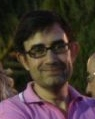
\includegraphics[width = 27
mm]{JJM.jpg},] \noindent\emph{JJ Merelo} es catedr\'{a}tico de Universidad
en el \'area de Arquitectura y Tecnolog\'{\i}a de Computadores, y
actualmente director de la Oficina de Software Libre de la UGR.
Mantiene un blog desde el a\~no 2002, y lo ha utilizado en clase desde
el a\~no 2004; tambi\'en wikis y, ultimamente, agregadores y otras
herramientas TIC. \'{U}ltimamente le ha dado por el \textsl{flipped
learning}, de lo que se informar\'{a} debidamente en esta columna.
\end{window}}}

\medskip

{\small{\begin{window}[0,r,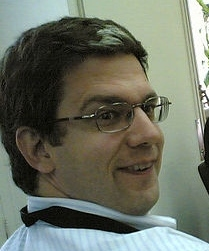
\includegraphics[width = 27 mm]{FTricas1.jpg},]
		\noindent  \emph{Fernando Tricas Garc\'{\i}a} es profesor
		titular de Lenguajes y Sistemas Inform\'aticos del Departamento
		de Inform\'atica e Ingenier\'{\i}a de Sistemas de la Universidad de
		Zaragoza.  Empez\'o a estudiar la blogosfera casi cuando a\'un no
		exist\'{\i}a (all\'a por el a\~no 2002) y a tratar de integrarla en los
		cursos y tareas docentes un poco despu\'es.  Ha impartido
		numerosas charlas relacionadas con el tema de la Web 2.0.
		Es actualmente Director de su departamento.  
		\end{window}}}
%-------------------------------------------------


\bigskip

\noindent\emph{Todas las columnas de la serie Docencia 2.0
pueden descargarse en formato LaTeX desde
{\small\url{https://github.com/ReVision-Docencia-20/Columnas}}}

\noindent\rule{90mm}{1pt}

{\small \noindent\copyright 2014 JJ. Merelo, F. Tricas. Este art\'{\i}culo es de acceso libre distribuido bajo los t\'erminos
de la Licencia Creative Commons de Atribuci\'on, que permite copiar,
distribuir y comunicar p\'ublicamente la obra en cualquier medio, s\'olido
o electr\'onico, siempre que se acrediten a los autores y fuentes
originales}

\end{multicols}
\end{document}
	








\end{multicols}
\end{document}
 
